% Weight diagrams of V_(2,1,0) and V_(3,0,0) of U(3). Generated by a short script.
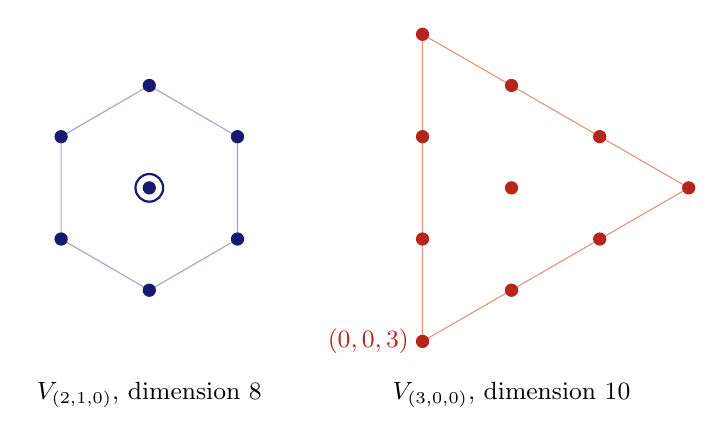
\begin{tikzpicture}[font=\small]
\draw[MidnightBlue!40] (1.12,0.65) -- (1.12,-0.65) -- (0.00,-1.30) -- (-1.12,-0.65) -- (-1.12,0.65) -- (0.00,1.30) -- cycle;
\fill[MidnightBlue] (-1.12,0.65) circle (2.4pt);
\fill[MidnightBlue] (0.00,1.30) circle (2.4pt);
\fill[MidnightBlue] (1.12,0.65) circle (2.4pt);
\fill[MidnightBlue] (1.12,-0.65) circle (2.4pt);
\fill[MidnightBlue] (-1.12,-0.65) circle (2.4pt);
\fill[MidnightBlue] (0.00,-1.30) circle (2.4pt);
\fill[MidnightBlue] (0.00,0.00) circle (2.4pt);
\draw[MidnightBlue,thick] (0.00,0.00) circle (5pt);
\node[below] at (0.00,-2.35) {$V_{(2,1,0)}$, dimension $8$};
\draw[BrickRed!40] (6.85,0.00) -- (3.47,1.95) -- (3.47,-1.95) -- cycle;
\fill[BrickRed] (3.47,-1.95) circle (2.4pt);
\fill[BrickRed] (3.47,-0.65) circle (2.4pt);
\fill[BrickRed] (3.47,0.65) circle (2.4pt);
\fill[BrickRed] (3.47,1.95) circle (2.4pt);
\fill[BrickRed] (4.60,-1.30) circle (2.4pt);
\fill[BrickRed] (4.60,0.00) circle (2.4pt);
\fill[BrickRed] (4.60,1.30) circle (2.4pt);
\fill[BrickRed] (5.72,-0.65) circle (2.4pt);
\fill[BrickRed] (5.72,0.65) circle (2.4pt);
\fill[BrickRed] (6.85,0.00) circle (2.4pt);
\node[BrickRed,left] at (3.42,-1.95) {$(0,0,3)$};
\node[below] at (4.60,-2.35) {$V_{(3,0,0)}$, dimension $10$};
\end{tikzpicture}
